\documentclass{article}
\usepackage[english]{babel}
\usepackage[utf8]{inputenc}
\usepackage[T1]{fontenc}
\usepackage{amsmath}
\usepackage[us]{datetime}
\usepackage{graphicx}
\usepackage[font=small,labelfont=bf]{caption}
\usepackage[font=small,labelfont=bf]{subcaption}
\usepackage{listings}
\usepackage{color}
\renewcommand{\lstlistingname}{Code}
\captionsetup[subfigure]{font=footnotesize}
\setlength{\parindent}{0in}


\author{Madis Ollikainen}
\title{Progress report: Learning vol2}

\begin{document}

\maketitle

%% For Stefanos comments %% 
%\section{Stefano's comment}
%{\color{red}I will write my comments in red, so that you can spot them easily.}

\section{New/updated learning schema}
I updated the learning schema such that after every time step each possible strategy for each player gets an updated value, based on the gain the player would have gotten if they would have played a specific strategy. 
The info about the value of each strategy is held in an array of doubles called \emph{memory}, which is of length $N_{agents} \times N_{strategies}$. All entries in \emph{memory} are initialised to $1$. After each round $t$ each agents $i$ updates its memory entries $M_ij$ for the all strategies $j$. The update $M_{ij}(t) \rightarrow M_{ij}(t+1)$ is done as
\[
M_{ij}(t+1) = M_{ij}(t)\left(1 + \xi\frac{gain_{ij}}{w_i(t-1)} \right), 
\]   
where $w_i(t-1)$ is the wealth of agent $i$ before round $t$ and $\xi$ is a pre-defined learning factor, which can be set in the configuration file under the \emph{mUpDate} variable. The $gain_{ij}$ is calculated from the knowledge of what other players did during the time step $t$. That mean, that after time step $t$ each player evaluates how well he would have done, if he would have chosen any of the strategies, keeping the choice of the other player fix to the ones they actually did.   

\vspace{10pt}

Before each round the strategies of all agents are updated (\emph{! the actual strategy being played !}) using the entries in the array memory array $M$. The updating schema has the same probabilistic structure as it had in the previous simulations. The probabilities of each strategy $j$ for agent $i$ are calculated as
\[
p_{ij} = \frac{e^{\beta M_{ij}}}{\sum_{k}e^{\beta M_{ik}}}.
\]

\vspace{10pt}

Test result for $\xi = \{0.1, 0.05, 0.01 \}$ using $N=1200$ players during $T = 50$ time steps are shown in the graphs below. A smaller $\xi$ value seems to slow the process of the $\alpha r$ ordering schema giving an unequal society. \emph{I'll run some longer simulations to see if this truly is like that.}

\break

%% New learning schema %% 
\begin{figure}[!htb]
\centering

% xi = 0.1 %

\begin{subfigure}[t]{0.333\textwidth}
\centering
\includegraphics[width=\textwidth]{{sml_LFO_N1200_E0.1_cooperation}.pdf}
\caption{Cooperation \\ $\xi = 0.1$}
\end{subfigure}%
%
\hfill
%
\begin{subfigure}[t]{0.333\textwidth}
\centering
\includegraphics[width=\textwidth]{{sml_LFO_N1200_E0.1_gini}.pdf}
\caption{Gini \\ $\xi = 0.1$}
\end{subfigure}%
%
\hfill
%
\begin{subfigure}[t]{0.333\textwidth}
\centering
\includegraphics[width=\textwidth]{{sml_LFO_N1200_E0.1_growth}.pdf}
\caption{Growth \\ $\xi = 0.1$}
\end{subfigure}%

\bigskip 

% xi = 0.05 %

\begin{subfigure}[t]{0.333\textwidth}
\centering
\includegraphics[width=\textwidth]{{sml_LFO_N1200_E0.05_cooperation}.pdf}
\caption{Cooperation \\ $\xi = 0.05$}
\end{subfigure}%
%
\hfill
%
\begin{subfigure}[t]{0.333\textwidth}
\centering
\includegraphics[width=\textwidth]{{sml_LFO_N1200_E0.05_gini}.pdf}
\caption{Gini \\ $\xi = 0.05$}
\end{subfigure}%
%
\hfill
%
\begin{subfigure}[t]{0.333\textwidth}
\centering
\includegraphics[width=\textwidth]{{sml_LFO_N1200_E0.05_growth}.pdf}
\caption{Growth \\ $\xi = 0.05$}
\end{subfigure}%

\bigskip

% xi = 0.01 %

\begin{subfigure}[t]{0.333\textwidth}
\centering
\includegraphics[width=\textwidth]{{sml_LFO_N1200_E0.01_cooperation}.pdf}
\caption{Cooperation \\ $\xi = 0.01$}
\end{subfigure}%
%
\hfill
%
\begin{subfigure}[t]{0.333\textwidth}
\centering
\includegraphics[width=\textwidth]{{sml_LFO_N1200_E0.01_gini}.pdf}
\caption{Gini \\ $\xi = 0.01$}
\end{subfigure}%
%
\hfill
%
\begin{subfigure}[t]{0.333\textwidth}
\centering
\includegraphics[width=\textwidth]{{sml_LFO_N1200_E0.01_growth}.pdf}
\caption{Growth \\ $\xi = 0.01$}
\end{subfigure}%

\bigskip

\caption{New learning schema results with $N = 1200$ players for $\xi = \{0.1, 0.05, 0.01\}$ during $50$ iterations.}
\end{figure}

\break

\section{Equal talent comparison}
I ran simulations with equal talent $1$ for each player for all three schemas: the new (NLS) and the old (OLS) learning and the Nash equilibrium. The simulations had $N=500$ players and lasted for $T=50$ time steps. 

%% Equal talen %% 
\begin{figure}[h]
\centering

% NLS  $\xi = 0.1$ %

\begin{subfigure}[t]{0.333\textwidth}
\centering
\includegraphics[width=\textwidth]{{ST_sml_LFO_N500_E0.1_cooperation}.pdf}
\caption{Cooperation \\ NLS  $\xi = 0.1$}
\end{subfigure}%
%
\hfill
%
\begin{subfigure}[t]{0.333\textwidth}
\centering
\includegraphics[width=\textwidth]{{ST_sml_LFO_N500_E0.1_gini}.pdf}
\caption{Gini \\ NLS  $\xi = 0.1$}
\end{subfigure}%
%
\hfill
%
\begin{subfigure}[t]{0.333\textwidth}
\centering
\includegraphics[width=\textwidth]{{ST_sml_LFO_N500_E0.1_growth}.pdf}
\caption{Growth \\ NLS  $\xi = 0.1$}
\end{subfigure}%

\bigskip 

% OLS  $\xi = 0.1$ %

\begin{subfigure}[t]{0.333\textwidth}
\centering
\includegraphics[width=\textwidth]{{ST_sml_N500_E0.1_cooperation}.pdf}
\caption{Cooperation \\ OLS  $\xi = 0.1$}
\end{subfigure}%
%
\hfill
%
\begin{subfigure}[t]{0.333\textwidth}
\centering
\includegraphics[width=\textwidth]{{ST_sml_N500_E0.1_gini}.pdf}
\caption{Gini \\ OLS  $\xi = 0.1$}
\end{subfigure}%
%
\hfill
%
\begin{subfigure}[t]{0.333\textwidth}
\centering
\includegraphics[width=\textwidth]{{ST_sml_N500_E0.1_growth}.pdf}
\caption{Growth \\ OLS  $\xi = 0.1$}
\end{subfigure}%

\bigskip

% Nash eq.  %

\begin{subfigure}[t]{0.333\textwidth}
\centering
\includegraphics[width=\textwidth]{{ST_nashEQ_N500_cooperation}.pdf}
\caption{Cooperation \\ Nash eq.}
\end{subfigure}%
%
\hfill
%
\begin{subfigure}[t]{0.333\textwidth}
\centering
\includegraphics[width=\textwidth]{{ST_nashEQ_N500_gini}.pdf}
\caption{Gini \\ Nash eq.}
\end{subfigure}%
%
\hfill
%
\begin{subfigure}[t]{0.333\textwidth}
\centering
\includegraphics[width=\textwidth]{{ST_nashEQ_N500_growth}.pdf}
\caption{Growth \\ Nash eq.}
\end{subfigure}%

\bigskip

\bigskip

\caption{All agents have talent $1$. NLS and OLS indicate the new and old learning schema correspondingly. Number of agents $N = 500$, simulation duration $T = 50$.}
\end{figure}

\break

\section{Nash eq blue line}
I also had to try and see why did the blue line (grouping according to the output) start falling at some point. It seems to me that for some reason this grouping method for the Nash equilibrium gives a rather jumpy growth and the falling effect was just a statistical feature. On the next page you can see the last twelve time steps for the grouping by output size. On those plots the size of the circles indicate the output size. It can be seen, that the position of the agents jumps around very much, due to which we also see a lot of jumping around for the growth plot in Fig 3 (c). 



%% Nash eq %% 
\begin{figure}[h]
\centering

% NLS  $\xi = 0.1$ %

\begin{subfigure}[t]{0.333\textwidth}
\centering
\includegraphics[width=\textwidth]{{nq_N500_cooperation}.pdf}
\caption{Cooperation}
\end{subfigure}%
%
\hfill
%
\begin{subfigure}[t]{0.333\textwidth}
\centering
\includegraphics[width=\textwidth]{{nq_N500_gini}.pdf}
\caption{Gini}
\end{subfigure}%
%
\hfill
%
\begin{subfigure}[t]{0.333\textwidth}
\centering
\includegraphics[width=\textwidth]{{nq_N500_growth}.pdf}
\caption{Growth}
\end{subfigure}%

\caption{Nash eq. simulation for $N=500$ during $T=50$ timesteps.}
\end{figure}



%% Nash eq JUMPY %% 
\begin{figure}[h]
\centering

% NLS  $\xi = 0.1$ %

\begin{subfigure}[t]{0.333\textwidth}
\centering
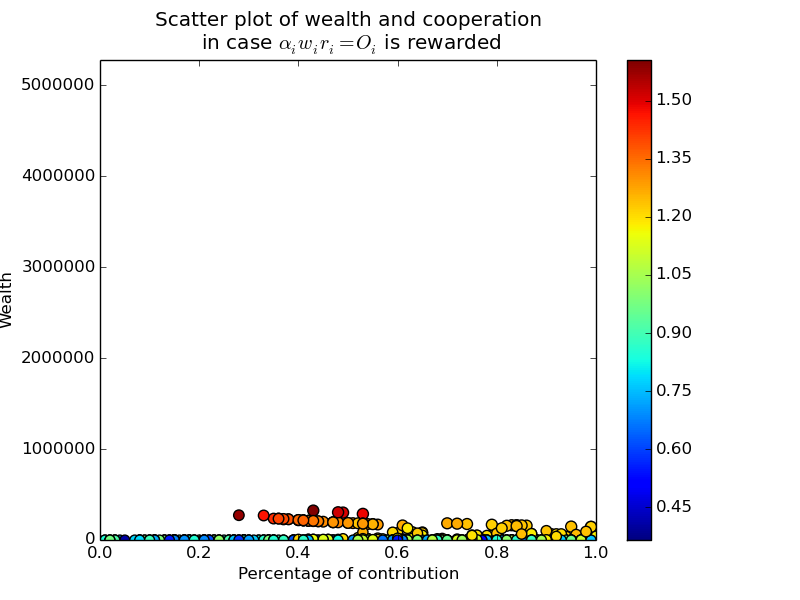
\includegraphics[width=\textwidth]{nq_output_scatter/scatter_ranking_1_039.png}
\caption{$T = 39$}
\end{subfigure}%
%
\hfill
%
\begin{subfigure}[t]{0.333\textwidth}
\centering
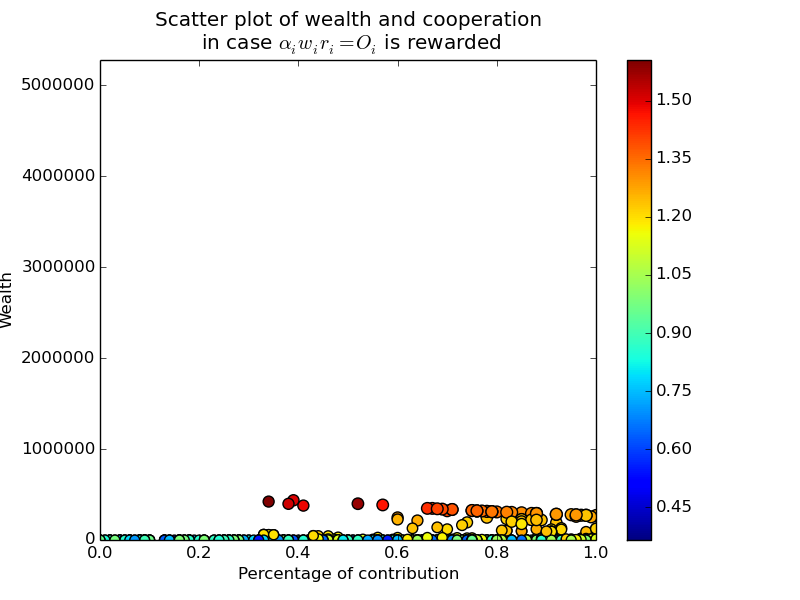
\includegraphics[width=\textwidth]{nq_output_scatter/scatter_ranking_1_040.png}
\caption{$T = 40$}
\end{subfigure}%
%
\hfill
%
\begin{subfigure}[t]{0.333\textwidth}
\centering
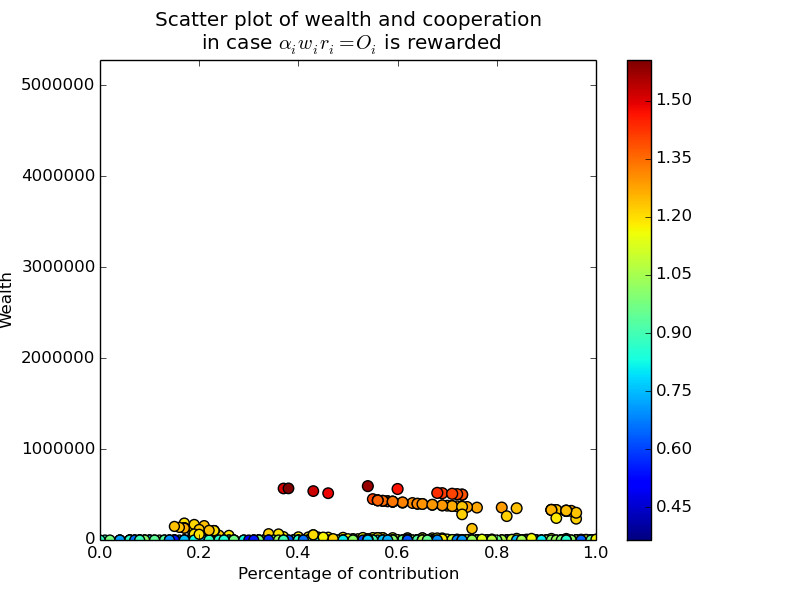
\includegraphics[width=\textwidth]{nq_output_scatter/scatter_ranking_1_041.png}
\caption{$T = 41$}
\end{subfigure}%

\bigskip

\begin{subfigure}[t]{0.333\textwidth}
\centering
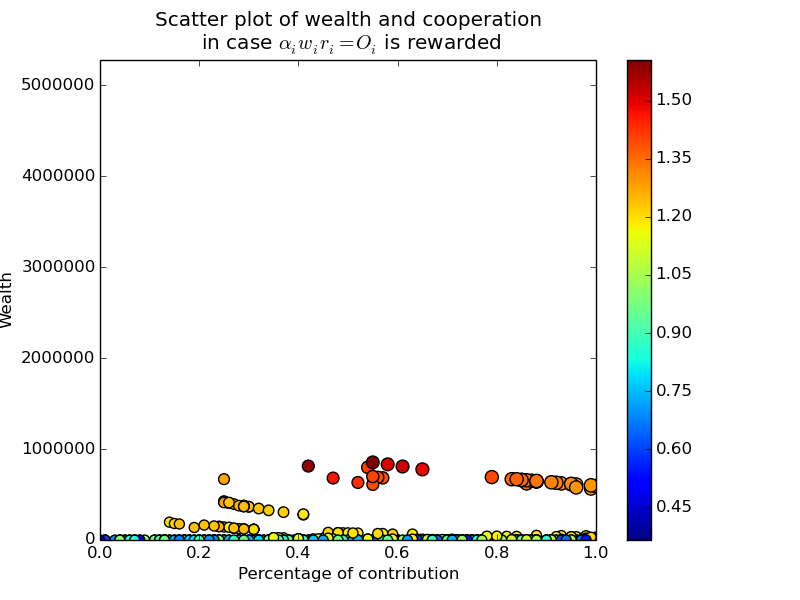
\includegraphics[width=\textwidth]{nq_output_scatter/scatter_ranking_1_042.png}
\caption{$T = 42$}
\end{subfigure}%
%
\hfill
%
\begin{subfigure}[t]{0.333\textwidth}
\centering
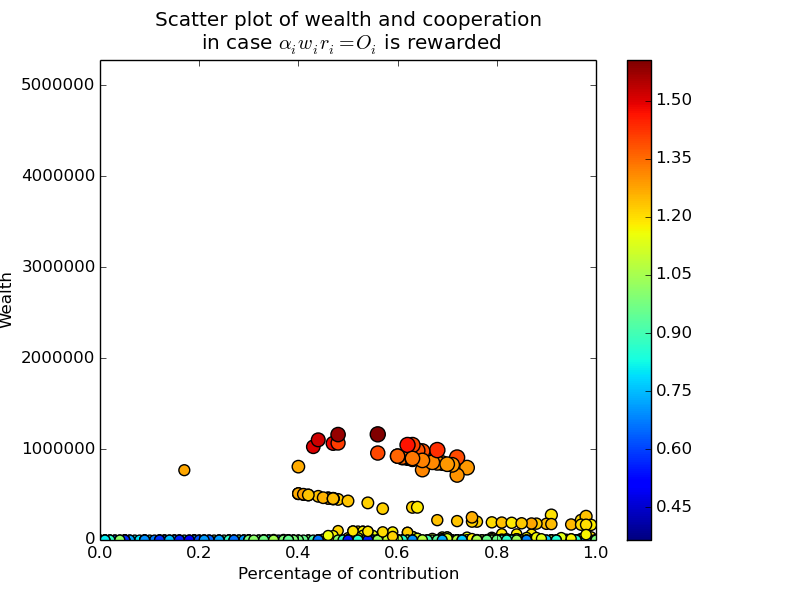
\includegraphics[width=\textwidth]{nq_output_scatter/scatter_ranking_1_043.png}
\caption{$T = 43$}
\end{subfigure}%
%
\hfill
%
\begin{subfigure}[t]{0.333\textwidth}
\centering
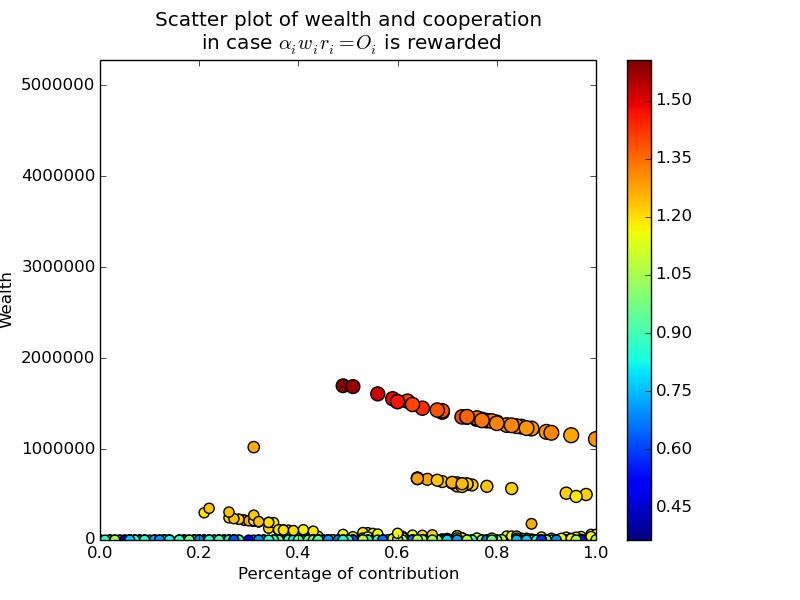
\includegraphics[width=\textwidth]{nq_output_scatter/scatter_ranking_1_044.png}
\caption{$T = 44$}
\end{subfigure}%

\bigskip


\begin{subfigure}[t]{0.333\textwidth}
\centering
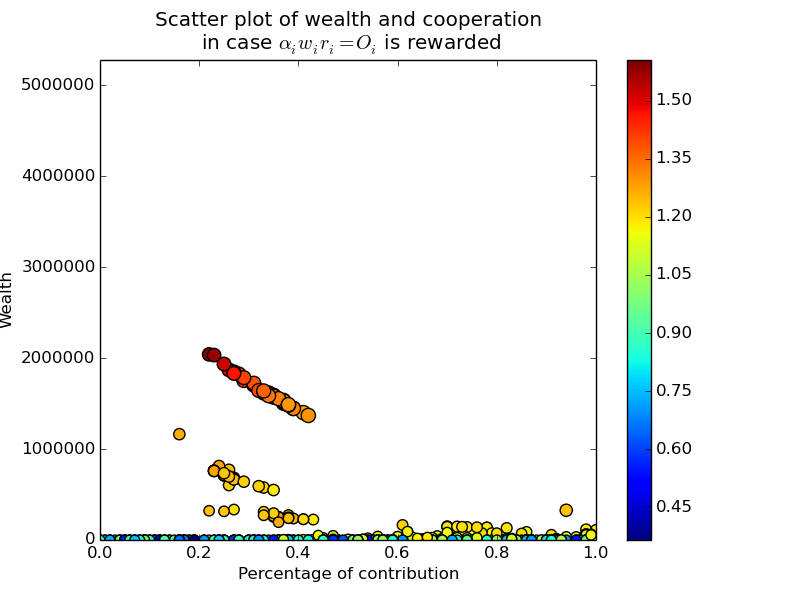
\includegraphics[width=\textwidth]{nq_output_scatter/scatter_ranking_1_045.png}
\caption{$T = 45$}
\end{subfigure}%
%
\hfill
%
\begin{subfigure}[t]{0.333\textwidth}
\centering
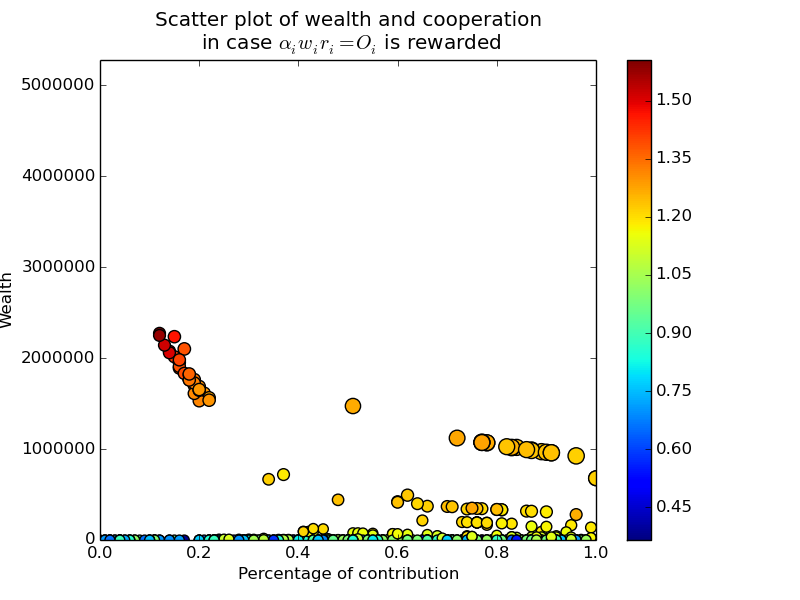
\includegraphics[width=\textwidth]{nq_output_scatter/scatter_ranking_1_046.png}
\caption{$T = 46$}
\end{subfigure}%
%
\hfill
%
\begin{subfigure}[t]{0.333\textwidth}
\centering
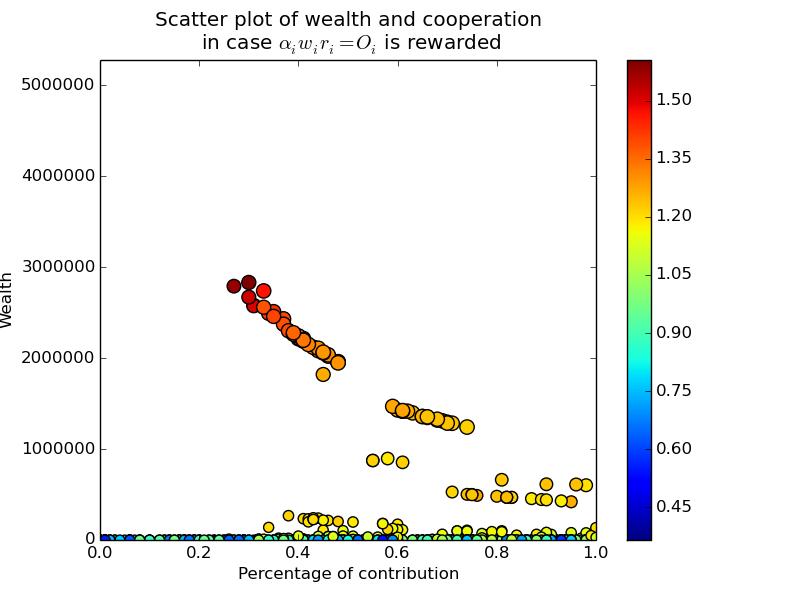
\includegraphics[width=\textwidth]{nq_output_scatter/scatter_ranking_1_047.png}
\caption{$T = 47$}
\end{subfigure}%

\bigskip

\begin{subfigure}[t]{0.333\textwidth}
\centering
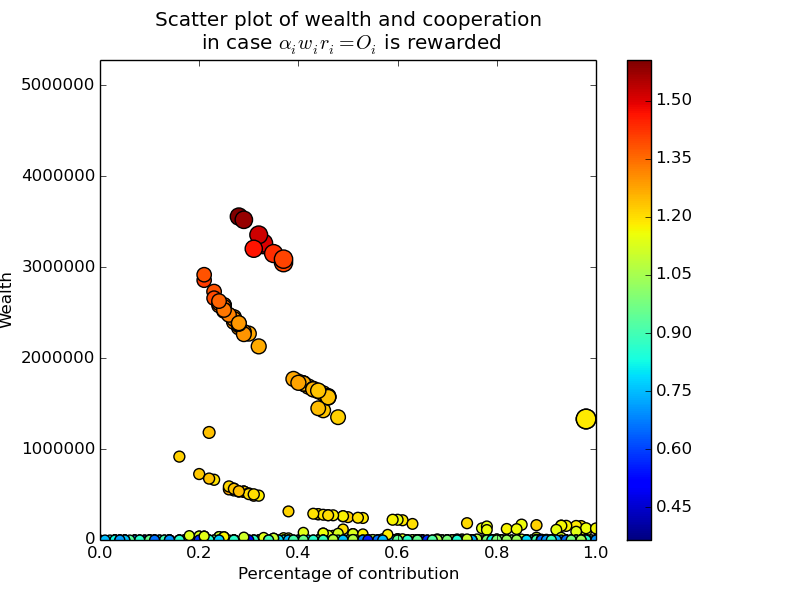
\includegraphics[width=\textwidth]{nq_output_scatter/scatter_ranking_1_048.png}
\caption{$T = 48$}
\end{subfigure}%
%
\hfill
%
\begin{subfigure}[t]{0.333\textwidth}
\centering
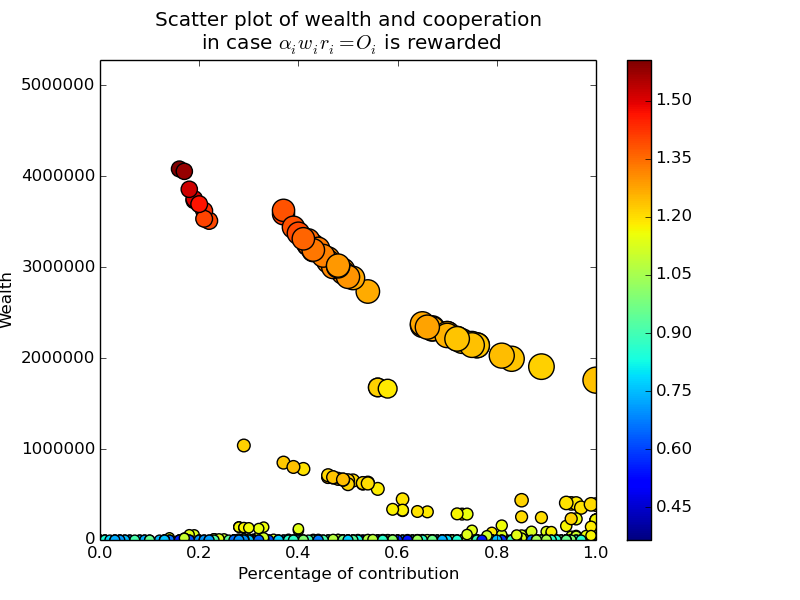
\includegraphics[width=\textwidth]{nq_output_scatter/scatter_ranking_1_049.png}
\caption{$T = 49$}
\end{subfigure}%
%
\hfill
%
\begin{subfigure}[t]{0.333\textwidth}
\centering
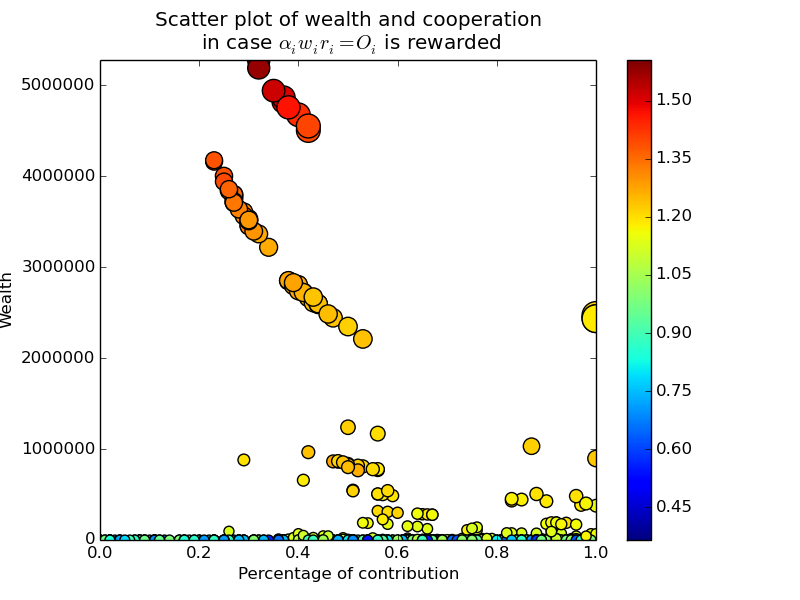
\includegraphics[width=\textwidth]{nq_output_scatter/scatter_ranking_1_050.png}
\caption{$T = 50$}
\end{subfigure}%


\bigskip

\caption{Nash eq. simulation for $N=500$ with grouping by the output value $O_i = \alpha_i r_i \omega_i$ for the twelve last time steps. The size of the circles indicate the value of the output.}
\end{figure}

\end{document}